%%%
%%% BACHELOR'S THESIS TEMPLATE - ENGLISH
%%%
%%%  * the third chapter
%%%
%%%  AUTHORS:  Arnost Komarek (komarek@karlin.mff.cuni.cz), 2011
%%%            Michal Kulich (kulich@karlin.mff.cuni.cz), 2013
%%%
%%%  LAST UPDATED: 20130318
%%%
%%%  ===========================================================================

\chapter{Descripci�n de im�genes}

\section{Recurrent Neural Networks - RNNs}

A diferencia de las redes neuronales tradicionales, en las redes neuronales recurrentes
se considera que los datos de entrada (y salida) no son independientes entre s�.
Entre los principales usos de estas redes destacamos dos:

\begin{enumerate}
\item Clasificar sentencias de acuerdo a su probabilidad de aparecer en una situaci�n real,
d�ndonos una medida de su correcci�n sint�ctica y/o gram�tica.
\item Generar texto nuevo (original) tras entrenar el sistema con frases de prueba.
\end{enumerate}

Observamos la importancia de considerar dependencias entre las entradas y las salidas de la red:
en el caso de las frases, si queremos generar una nueva palabra, tendremos que tener en cuenta
la parte de la frase ya generada, pues esta influir� en el resto de la sentencia.

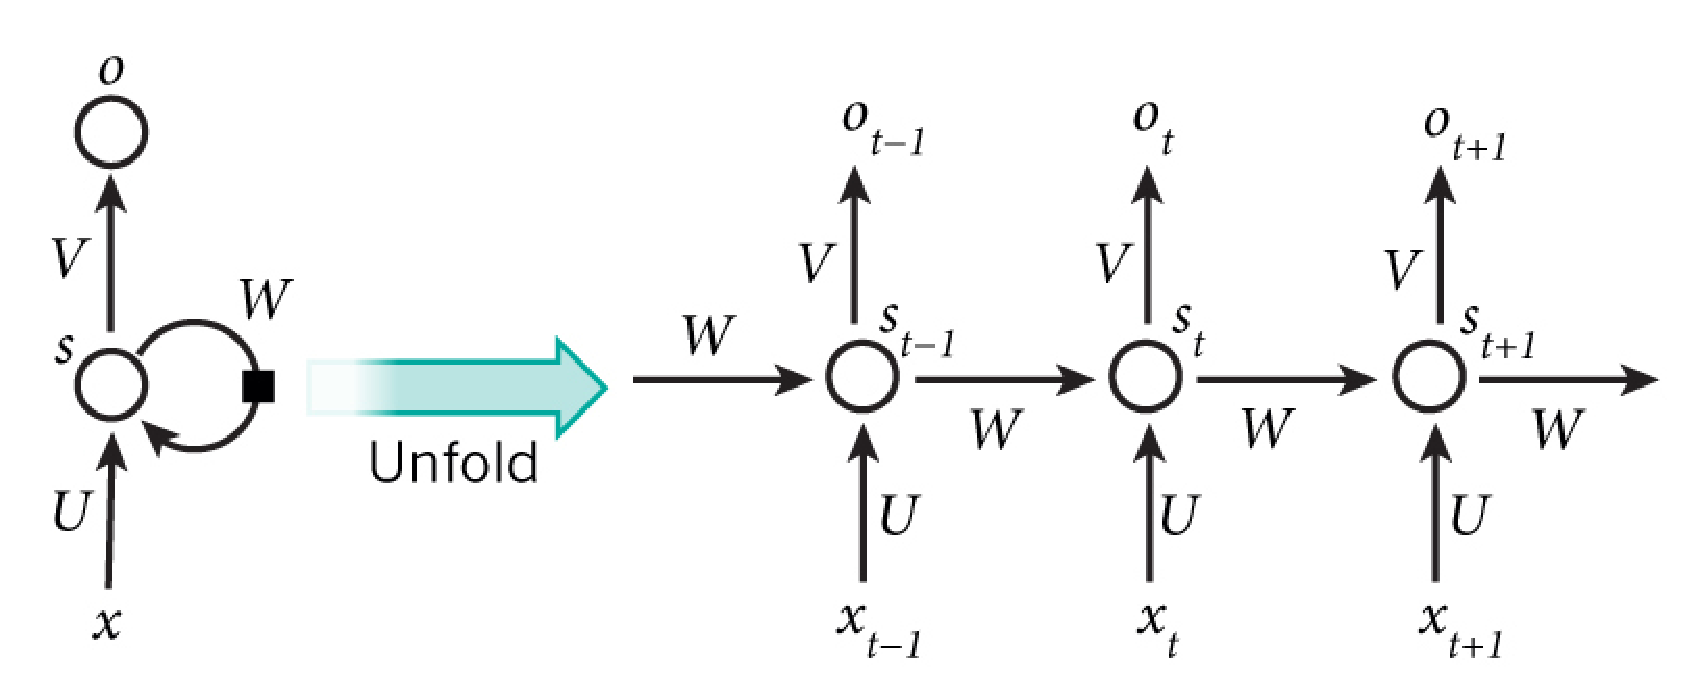
\includegraphics[width=\linewidth]{\FIGDIR/rnn.eps}

En este caso, $x_t$ representa la entrada de la red, $s_t$ el estado oculto y $o_t$
la salida en el paso $t$. En la figura vemos que el estado $s_t$ se calcula como
funci�n del estado anterior $s_{t-1}$, la entrada en el paso actual $x_t$.
La red posee "memoria" en el sentido en que los estados anteriores condicionan
el estado actual. Sin embargo, esta memoria no se mantiene durante muchas fases.
Existe un tipo concreto de RNN, las conocidas como \textit{long short-term memory}
(LSTM) que favorece la persistencia de los datos de los estados anteriores durante
un n�mero de mayor de fases, lo que las hace especialmente indicadas para comprensi�n
de lenguaje natural, an�lisis de textos manuscritos y reconocimiento de voz.

\section{Convolutional Neural Networks - CNNs}

Las redes neuronales convolutivas se utilizan en tareas como la clasificaci�n y reconocmiento de im�genes.

%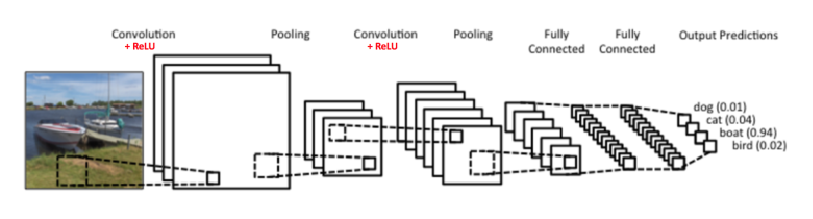
\includegraphics[width=\linewidth]{\FIGDIR/cnn.eps}

Podemos ver que el modelo asigna la mayor probabilidad a "barco" de entre las cuatro
categor�as existentes. En el modelo de la figura observamos cuatro operaciones en la red:

\begin{itemize}
\item \textbf{Convoluci�n.} El principal objetivo de la operaci�n de convoluci�n
es extraer caracter�sticas de una imagen.La convoluci�n preserva la relaci�n
espacial entre los pixels de la imagen usando peque�os cuadros como datos de entrada.

\includegraphics[width=\linewidth]{\FIGDIR/convolution.eps}

Consideramos una imagen como una matriz bidimensional de p�xeles (input), y otra
 matriz (\textit{kernel} o filtro), normalmente de tama�o $3x3$ que "recorre" la
 imagen de entrada. Con los valores del kernel y la porci�n de imagen que cubre,
 se computa la convoluci�n y esto da como resultado otra imagen (mapa de activaci�n).

\item \textbf{No linealidad.} Se aplica una funci�n de activaci�n no lineal operando
sobre cada pixel del mapa de activaci�n. Aunque pueden usarse funciones como la
sigmoide, se ha probado que la funci�n ReLU (Rectified Linear Unit) da mejores
resultados en este tipo de redes neuronales [REF].

%
\includegraphics[width=\linewidth]{\FIGDIR/relu.eps}

\item \textbf{Pooling.} Se encarga de reducir el tama�o del mapa de activaci�n
conservando los elementos m�s importantes. El \textit{Pooling} puede ser de
distintos tipos: Max, Sum, Avg...

%
\includegraphics[width=\linewidth]{\FIGDIR/maxpool.eps}

En el caso del \textit{Max Pooling}, se define un espacio (por ejemplo una matriz
 $2x2$) y para cada bloque $2x2$ se coge el mayor valor de entre los 4 existentes.

La funci�n del \textit{Pooling} es reducir las im�genes y convertirlas en objetos
 m�s manejables por las siguientes capas de la red.

\item \textbf{Fully Connected Layer.} Tras la convoluci�n y el \textit{Pooling},
obtenemos caracter�sticas de alto nivel de la imagen de entrada. En esta fase, y
usando dichas caracter�sticas como entrada, clasificamos la imagen en una serie
de categor�as basadas en el \textit{dataset} de entrenamiento.


\includegraphics[width=\linewidth]{\FIGDIR/fullycon.eps}

\end{itemize}
